%!TEX root = ../crimson_throne_book_main.tex
% 2016-05-07
The companions consider what to do. Should they dive into the library and look for more information on Shoanti graves? Is there a way they can bring Zellara back? Should they try and contact the resistance? Are the many young girls who are being recruited for the Maidens in need of rescue? And what should they use for an excuse if they need a good cover story? Mixing truth with fiction, they decide upon a tale that they have to return the ancient bones of a mythic shaman to the Shoanti to keep them from invading Korvosa with a huge army.\\

Maybe it is best to start with something easy first: suspecting that Vencarlo is hiding in Old Korvosa, the party heads for the island in the north of the city. When they cross Jeggare Circle, they happen upon the construction of a gigantic statue of the queen from black stones. The laborers seem little motivated, as do the members of the Korvosan Guard who have been tasked to watch over the site. The stone reaches twenty feet already, and it looks like it only goes up to Ileosa's knees so far.\\

The only bridge over the Narrows of Saint Alika has a guard detail of Gray Maidens and all who want to cross are given a thorough inspection. The party goes west, wanting to get over the water at the westernmost point of the Narrows with the {\itshape Dimension Door} from Puk's cloak. When they get there, they find out where the big black stones for Ileosa's statue come from: the Great Tower is being torn down. A magic jump brings the companions to the other side of the water, to some of the poorest quarters of Old Korvosa. The upside of this poverty-stricken neighborhood is that it is almost free of Gray Maidens, making it easy for the party to get to House Arkona. Glorio Arkona welcomes the heroes with open arms, once again offering to aid them in their quest to fight the evil in Castle Korvosa and inviting them to stay in his house, since their villa has been compromised. Sjo thanks him for his kindness, but says they have their own place to lay low. Lord Arkona denies being involved with the resistance, claiming the rebels are hiding somewhere in the south of the city. He hasn't seen Vencarlo since he left the city and didn't even know the fencing master had returned. When Quint tells him about the Red Mantis attacks, Glorio is worried. The assassins are not known for giving up, once the mantis are on your tail, they do not relent. The heroes confront Glorio with their own dilemma: they need to recover the bones of an old Shoanti shaman who was buried somewhere in the city long ago. What would be the best way to find his grave: magic or research in the library? Lord Arkona is not sure, but reckons that magic would definitely be easier. Still, Quint cannot think of an effective spell that would lead him to his goal in due time.\\

Finally the companions decide to check out the library. Quint tries to come up with a plan to infiltrate the occupied building, perhaps in the guise of some official who is on a royal mission. That might suffice to fool the Gray Maidens. The best course of action would be to stake out the place first. When darkness has fallen, Lord Arkona has the party taken back to the mainland in a small boat, but not after hosting an exotic dinner party and extending a helping hand once more for the future. By the light of the moon the party walks past the Acadamae; nothing can be seen beyond its great walls, except for the imps who flutter in the air above.\\

House Leroung is situated in the heart of Korvosa, on the university grounds.\hyperref[fig:House-Leroung-in-Curse-of-the-Crimson-Throne-607543444]{ The splendid manor in gothic style houses the city's biggest library on one side, and the family's living quarters on the other } . Since the nobles are under house arrest, they might have ample time to do research for the companions, so Balian wonders if they would be able to contact one of them and enlist their aid, like Aisha, the star from  {\itshape The Passion of Saint Alika} , or professor Sirtane, the alchemist who cured the plague. \\

\begin{figure}[h]
	\centering
	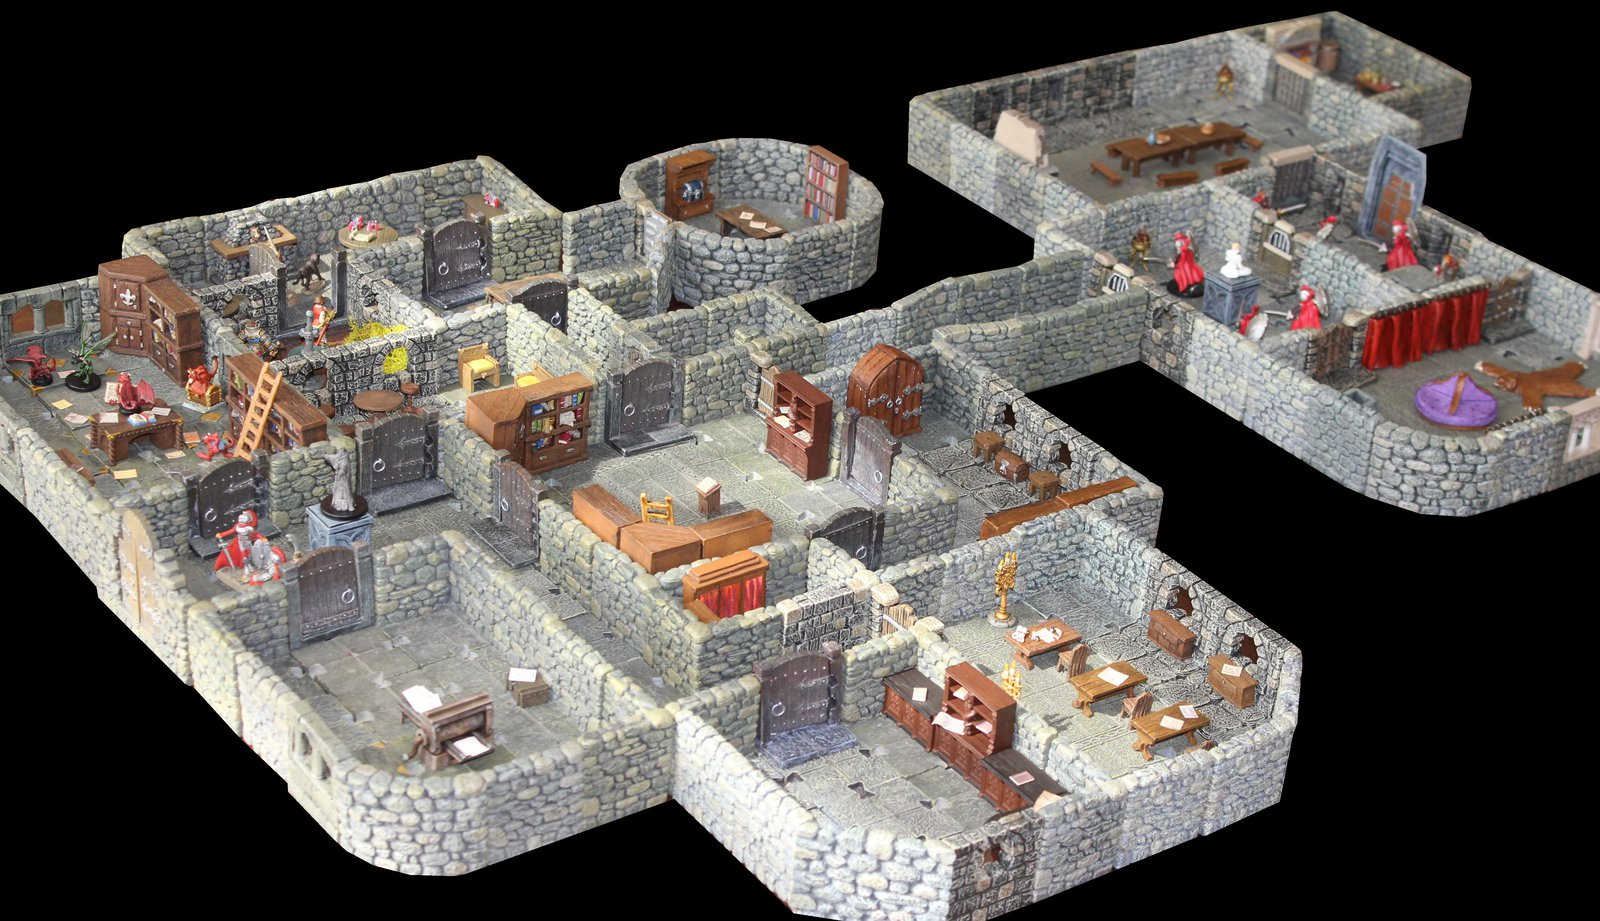
\includegraphics[width=0.39\textwidth]{images/House-Leroung-in-Curse-of-the-Crimson-Throne-607543444.jpg}
	\caption{House Leroung in Curse of the Crimson Throne}
	\label{fig:House-Leroung-in-Curse-of-the-Crimson-Throne-607543444}
\end{figure}

Puk circles the building, picking up noise and laughter from the corner room. Balian activates his {\itshape flying} boots and peeks inside, but the room is unlit, so the ranger cannot see a thing. Sjo remembers that Sirtane Leroung's laboratory led out into a small patio area. This might be the perfect way inside. Balian flies everyone over and Puk tries to pick the lock, but finds it too hard to open. Quint pulls out the Key-Lock Killer's bell and manages to get the way in unlocked. \hyperref[fig:Sneaking-into-House-Leroung-607544485]{ The heroes sneak inside } and reach the central library, where books on history are stored. Quint wonders whether they should look through the books themselves rather than bother the family, but the party's conversation alerts the two Gray Maidens who are guarding the public entrance. Apparently our friends forgot that you always have to keep quiet in the library. \hyperref[fig:Busted-in-House-Leroung-607546219]{ The female soldiers are not pleased at finding the nightly intruders } , but Quint uses his bardic power of persuasion to convince them that he and his friends are on an important mission. They need to talk to one of the Leroungs urgently. His deception works and the guards lead the party to the other side of the building, where the Leroungs live. Unfortunately there are even more Gray Maidens in this part of the house, who do not succumb to Quint's mind games. They draw steel, threatening to drown the room, a private shrine to Irori, in blood. \\

\begin{figure}[h]
	\centering
	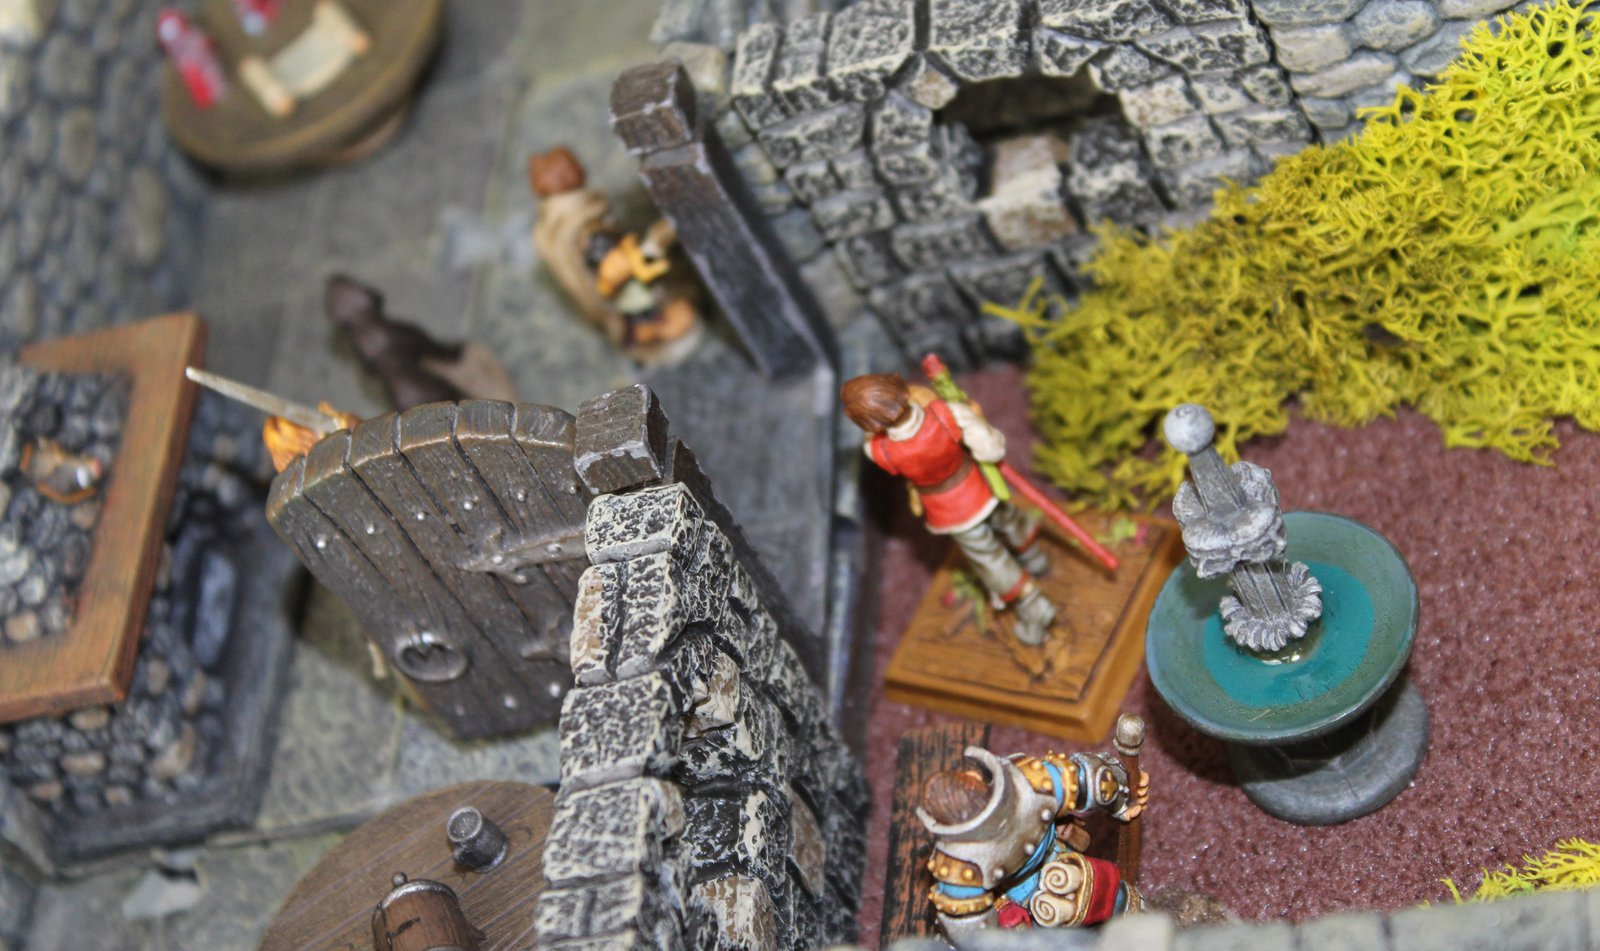
\includegraphics[width=0.39\textwidth]{images/Sneaking-into-House-Leroung-607544485.jpg}
	\caption{Sneaking into House Leroung}
	\label{fig:Sneaking-into-House-Leroung-607544485}
\end{figure}

\begin{figure}[h]
	\centering
	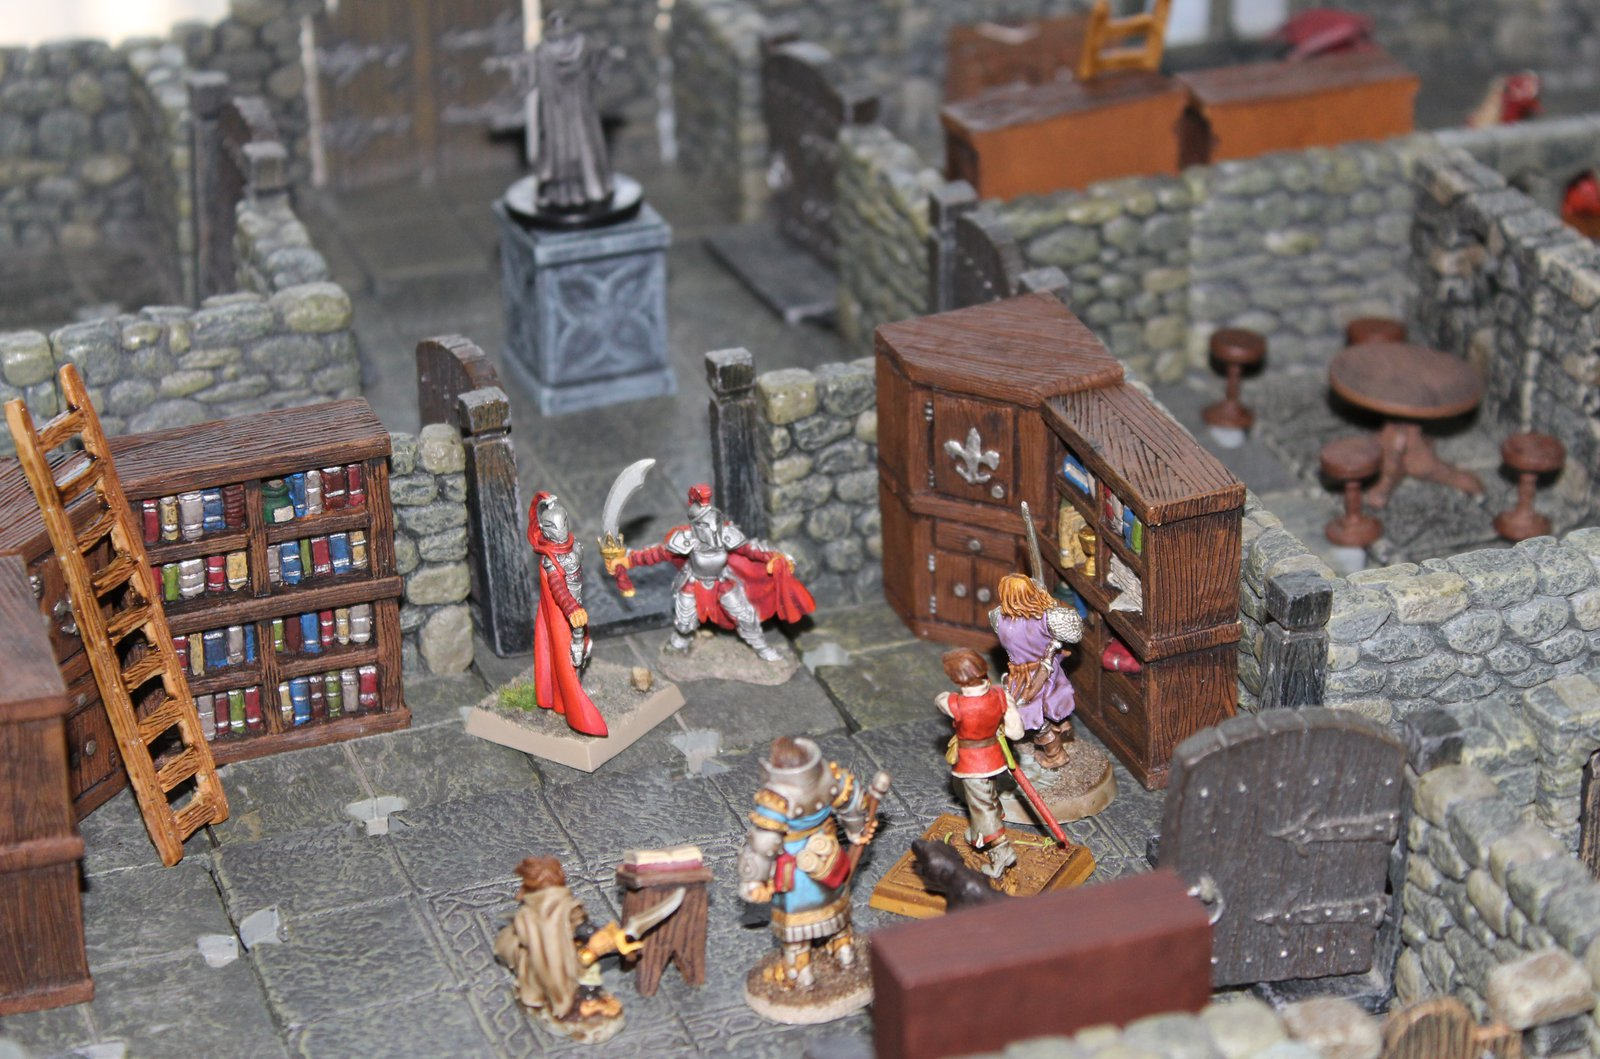
\includegraphics[width=0.39\textwidth]{images/Busted-in-House-Leroung-607546219.jpg}
	\caption{Busted in House Leroung}
	\label{fig:Busted-in-House-Leroung-607546219}
\end{figure}

